% boilert — Installation Manual
% Build with: latexmk -pdf installation-manual.tex
\documentclass[11pt,a4paper,parskip=half]{scrartcl}

% ---------------------------------------------------------------------------
% Fonts & encoding (pdflatex)
% ---------------------------------------------------------------------------
\usepackage[T1]{fontenc}
\usepackage[utf8]{inputenc}
\usepackage{lmodern}
\usepackage{tgheros}
\renewcommand{\familydefault}{\sfdefault}
\usepackage{microtype}

% ---------------------------------------------------------------------------
% Layout
% ---------------------------------------------------------------------------
\usepackage[a4paper,margin=2.4cm,bottom=3cm]{geometry}
\usepackage[english]{babel}
\usepackage{csquotes}
\usepackage{enumitem}
\setlist{itemsep=2pt,topsep=4pt}

% ---------------------------------------------------------------------------
% Colors — matching the application theme
% ---------------------------------------------------------------------------
\usepackage{xcolor}
\definecolor{accent}{HTML}{1C5CAB}      % primary blue
\definecolor{accentlight}{HTML}{3987E5} % series blue
\definecolor{hotred}{HTML}{E0442E}
\definecolor{warmamber}{HTML}{B7791F}
\definecolor{coldblue}{HTML}{2E7CD6}
\definecolor{okgreen}{HTML}{0B7A0B}
\definecolor{inkdark}{HTML}{1A1A19}
\definecolor{inkgray}{HTML}{52514E}
\definecolor{panelbg}{HTML}{F4F6F9}

% KOMA headings in the accent color
\addtokomafont{section}{\color{accent}}
\addtokomafont{subsection}{\color{accent}}
\addtokomafont{subsubsection}{\color{inkdark}}

% ---------------------------------------------------------------------------
% Header / footer
% ---------------------------------------------------------------------------
\usepackage[headsepline]{scrlayer-scrpage}
\clearpairofpagestyles
\ihead{\color{inkgray}\small boilert --- Installation Manual}
\ohead{\color{inkgray}\small v\boilertversion}
\ofoot{\color{inkgray}\small\pagemark}
\setkomafont{headsepline}{\color{accent!40}}

\newcommand{\boilertversion}{1.3.1}

% ---------------------------------------------------------------------------
% Graphics & diagrams
% ---------------------------------------------------------------------------
\usepackage{graphicx}
\graphicspath{{../}}
\usepackage{tikz}
\usetikzlibrary{positioning,arrows.meta,calc,shadows.blur}
\usepackage[europeanresistors]{circuitikz}
\usepackage{booktabs}
\usepackage{array}
\usepackage{tabularx}

% ---------------------------------------------------------------------------
% Boxes
% ---------------------------------------------------------------------------
\usepackage[most]{tcolorbox}
\newtcolorbox{note}[1][]{%
  enhanced,breakable,colback=accent!6,colframe=accent,
  boxrule=0pt,leftrule=3pt,arc=1.5mm,
  fonttitle=\bfseries,title={Note},#1}
\newtcolorbox{warningbox}[1][]{%
  enhanced,breakable,colback=warmamber!8,colframe=warmamber,
  boxrule=0pt,leftrule=3pt,arc=1.5mm,
  fonttitle=\bfseries,title={Warning},#1}
\newtcolorbox{tip}[1][]{%
  enhanced,breakable,colback=okgreen!7,colframe=okgreen,
  boxrule=0pt,leftrule=3pt,arc=1.5mm,
  fonttitle=\bfseries,title={Tip},#1}

% ---------------------------------------------------------------------------
% Code listings
% ---------------------------------------------------------------------------
\usepackage{listings}
\lstset{
  basicstyle=\ttfamily\small,
  backgroundcolor=\color{panelbg},
  frame=single, framerule=0pt, framesep=6pt,
  breaklines=true, upquote=true,
  showstringspaces=false,
  keywordstyle=\color{accent}\bfseries,
  commentstyle=\color{inkgray}\itshape,
  stringstyle=\color{okgreen},
  aboveskip=8pt, belowskip=8pt,
}
\lstdefinelanguage{toml}{
  comment=[l]{\#},
  morekeywords={},
  morestring=[b]{"},
}
\newcommand{\code}[1]{\texttt{#1}}

\usepackage[hidelinks,pdftitle={boilert Installation Manual},pdfauthor={boilert project}]{hyperref}

% ===========================================================================
\begin{document}

% ---------------------------------------------------------------------------
% Title page
% ---------------------------------------------------------------------------
\begin{titlepage}
  \centering
  \vspace*{1.2cm}
  % Decorative tank icon
  \begin{tikzpicture}[scale=1.1]
    \shade[top color=hotred!85, bottom color=coldblue!75, rounded corners=14pt,
           blur shadow={shadow blur steps=6}]
      (0,0) rectangle (2.2,3.4);
    \draw[rounded corners=14pt, inkgray!70, line width=1pt] (0,0) rectangle (2.2,3.4);
    % pipes
    \draw[line width=2.4pt, hotred!80]  (1.7,3.4) -- (1.7,3.8) -- (2.7,3.8);
    \draw[line width=2.4pt, coldblue!80] (0.5,0) -- (0.5,-0.4) -- (-0.5,-0.4);
    % sensors
    \foreach \y in {0.4,0.94,1.48,2.02,2.56,3.1} {
      \fill[white] (2.2,\y) circle (1.6pt);
      \draw[inkgray!80, line width=0.7pt] (2.2,\y) -- (2.55,\y);
    }
  \end{tikzpicture}

  \vspace{1.4cm}
  {\color{accent}\Huge\bfseries boilert}\\[0.35cm]
  {\Large\color{inkdark} Water Boiler Heat Monitor}\\[1.1cm]
  {\color{inkgray}\rule{0.55\textwidth}{0.6pt}}\\[1.1cm]
  {\huge\bfseries Installation Manual}\\[0.6cm]
  {\large Hardware -- Software -- Commissioning}\\[2.2cm]

  \begin{tabular}{rl}
    \textbf{Version} & \boilertversion\\[2pt]
    \textbf{Date} & July 2026\\[2pt]
    \textbf{Source} & \url{https://github.com/guycorbaz/boilert}\\
  \end{tabular}

  \vfill
  {\color{inkgray}\small For a Raspberry~Pi with the official 7\," touchscreen\\
   and DS18B20 1-Wire temperature sensors}
  \vspace*{1cm}
\end{titlepage}

\tableofcontents
\clearpage

% ===========================================================================
\section{Introduction}
% ===========================================================================

\textbf{boilert} estimates the amount of thermal energy stored in a cylindrical
domestic hot water tank. Between one and six DS18B20 temperature sensors are
attached to the tank wall, evenly spaced along its height; each sensor is
assumed to represent an equal horizontal slice of the water volume. The
application displays the temperatures, the computed energy and their 24-hour
history on the touchscreen, and publishes every measurement to an MQTT broker
for integration with a home automation system.

\subsection{System architecture}

\begin{center}
\begin{tikzpicture}[
    font=\small,
    box/.style={draw=accent, fill=accent!6, rounded corners=2mm,
                minimum height=1.5cm, align=center, line width=0.8pt},
    lbl/.style={font=\scriptsize\itshape, color=inkgray},
    flow/.style={-{Stealth[length=2.6mm]}, line width=0.9pt, color=inkdark}]
  \node[box, minimum width=2.6cm] (sensors) {DS18B20\\sensors ($\leq 6$)};
  \node[box, minimum width=3.4cm, right=1.6cm of sensors]
    (pi) {Raspberry Pi\\\textbf{boilert} + 7\," display};
  \node[box, minimum width=2.6cm, right=1.6cm of pi] (broker) {MQTT\\broker};
  \node[box, minimum width=2.6cm, right=1.4cm of broker, draw=inkgray,
        fill=panelbg] (ha) {Home\\automation};
  \draw[flow] (sensors) -- node[above, lbl]{1-Wire bus} (pi);
  \draw[flow] (pi) -- node[above, lbl]{MQTT} (broker);
  \draw[flow, color=inkgray, dashed] (broker) -- (ha);
\end{tikzpicture}
\end{center}

\subsection{How the energy is calculated}

Each valid sensor $i$ represents a slice of volume $V/N$ (tank volume divided
by the number of sensors). The stored energy above the cold-water reference
temperature $T_{\mathrm{ref}}$ is:
\[
  E\;[\mathrm{kWh}] \;=\; \frac{1}{1000}\sum_{i=1}^{N}
    \frac{V}{N}\;\cdot\;
    \max\bigl(0,\;T_i - T_{\mathrm{ref}}\bigr)\;\cdot\; c
\]
where $c = 1.162~\mathrm{Wh/(l\cdot K)}$ for water. Accuracy therefore depends
directly on \emph{even sensor spacing} and \emph{good thermal contact} --- the
two points this manual insists on.

% ===========================================================================
\section{Bill of materials}
% ===========================================================================

\begin{center}
\begin{tabularx}{\textwidth}{@{}lXl@{}}
\toprule
\textbf{Qty} & \textbf{Item} & \textbf{Remark}\\
\midrule
1 & Raspberry Pi (3B+ or newer recommended) & With power supply\\
1 & Official 7\," touchscreen (800\,$\times$\,480) & Or any 800$\times$480 display\\
1--6 & DS18B20 sensors, waterproof probe version & Stainless sleeve, 1--3\,m cable\\
1 & Resistor 4.7\,k$\Omega$, 1/4\,W & Single pull-up for the whole bus\\
-- & Wire, 3 conductors (e.g.\ 0.5\,mm$^2$) & Length: tank $\rightarrow$ Pi\\
-- & Screw terminals or solder + heat-shrink & Bus junctions\\
1 & Aluminium adhesive tape + thermal paste & Sensor mounting\\
-- & Cable ties / stainless hose clamps & Sensor fixation\\
1 & MicroSD card ($\geq$ 8\,GB) & Raspberry Pi OS\\
\bottomrule
\end{tabularx}
\end{center}

\begin{note}
An MQTT broker (e.g.\ Mosquitto) must be reachable on the network. It can run
on the same Raspberry Pi, on a NAS, or inside Home Assistant.
\end{note}

\begin{tip}[title={Dedicated interface PCB}]
Instead of the hand-wired pull-up resistor and screw terminals, you can use
the \textbf{1-Wire interface board} designed for this project:
\url{https://github.com/guycorbaz/1wire_raspi_pcb}. It is an open-hardware
KiCad~9 project that plugs onto the 40-pin GPIO header and provides Molex
Micro-Fit~3.0 connectors for the probes and an external supply, with the bus
pull-up and supply filtering already on board.
\end{tip}

% ===========================================================================
\section{Hardware installation}
% ===========================================================================

\subsection{Sensor placement on the tank}
\label{sec:placement}

The energy model divides the tank into $N$ horizontal slices of equal volume.
Each sensor must measure the temperature at the \emph{center} of its slice:
for a tank of height $H$ and $N$ sensors, sensor $i$ (counted from the top)
is placed at depth
\[
  d_i = \frac{(2i-1)\,H}{2N} \qquad\text{from the top of the water volume.}
\]
For the typical case $N=6$: $d = H/12,\ 3H/12,\ 5H/12,\ 7H/12,\ 9H/12,\ 11H/12$.

\begin{center}
\begin{tikzpicture}[font=\small, scale=0.9]
  % Tank body
  \shade[top color=hotred!75, bottom color=coldblue!70, rounded corners=16pt]
    (0,0) rectangle (3.2,7.2);
  \draw[rounded corners=16pt, inkgray, line width=1pt] (0,0) rectangle (3.2,7.2);
  % Insulation hint
  \draw[rounded corners=18pt, inkgray!50, line width=0.6pt, dashed]
    (-0.25,-0.25) rectangle (3.45,7.45);
  \node[color=inkgray, font=\scriptsize, rotate=90] at (-0.55,3.6) {insulation};
  % Pipes
  \draw[line width=3pt, hotred!85] (2.5,7.2) -- (2.5,7.9) -- (4.1,7.9);
  \node[right, color=hotred!90, font=\scriptsize] at (4.1,7.9) {hot water out};
  \draw[line width=3pt, coldblue!85] (0.7,0) -- (0.7,-0.7) -- (4.1,-0.7);
  \node[right, color=coldblue!90, font=\scriptsize] at (4.1,-0.7) {cold water in};
  % Height marks
  \draw[{Stealth[length=2mm]}-{Stealth[length=2mm]}, inkgray] (-1.35,0) -- (-1.35,7.2)
    node[midway, left, font=\scriptsize] {$H$};
  % Sensors at (2i-1)H/12 from top; H=7.2 => step 0.6
  \foreach \i/\d in {1/0.6, 2/1.8, 3/3.0, 4/4.2, 5/5.4, 6/6.6} {
    \fill[inkdark] (3.2,{7.2-\d}) circle (2pt);
    \draw[inkdark, line width=0.8pt] (3.2,{7.2-\d}) -- (3.8,{7.2-\d});
    \node[right, font=\scriptsize] at (3.8,{7.2-\d}) {\textbf{T\i}\; at $d_{\i}=\frac{\pgfmathparse{int(2*\i-1)}\pgfmathresult}{12}H$};
  }
  % Slice separators
  \foreach \y in {1.2,2.4,3.6,4.8,6.0} {
    \draw[white, dashed, line width=0.5pt, opacity=0.75] (0.05,\y) -- (3.15,\y);
  }
\end{tikzpicture}
\end{center}

Mounting each sensor:
\begin{enumerate}
  \item Remove the insulation locally to expose the bare steel wall.
  \item Apply a dab of thermal paste, press the stainless probe flat against
        the wall (along the wall, not perpendicular).
  \item Fix it with aluminium adhesive tape (which also spreads the heat), a
        hose clamp or a cable tie around the tank.
  \item Put the insulation back over the sensor. A probe left in open air
        reads the room, not the water.
\end{enumerate}

\begin{warningbox}
The order matters: the \emph{first} sensor in \code{config.toml} must be the
\emph{highest} probe on the tank, the last one the lowest. The stratification
display and the energy model both rely on this top-to-bottom ordering.
\end{warningbox}

\subsection{Wiring the 1-Wire bus}
\label{sec:wiring}

All sensors share the same three wires: \textbf{GND}, \textbf{DQ} (data) and
\textbf{3.3\,V}. A single 4.7\,k$\Omega$ pull-up resistor between DQ and
3.3\,V serves the whole bus. Waterproof DS18B20 probes almost always use:
red $=$ 3.3\,V, black $=$ GND, yellow (or white/blue) $=$ DQ.

\begin{center}
\begin{circuitikz}[font=\small, line width=0.8pt]
  % Raspberry Pi
  \draw[rounded corners=2mm, fill=accent!6, draw=accent]
    (0,0) rectangle (3.2,4.2);
  \node[align=center, color=accent] at (1.6,3.6) {\textbf{Raspberry Pi}\\GPIO header};
  \node[right, font=\scriptsize] at (0.15,2.8) {pin 1 --- 3.3\,V};
  \node[right, font=\scriptsize] at (0.15,1.8) {pin 7 --- GPIO4 (DQ)};
  \node[right, font=\scriptsize] at (0.15,0.8) {pin 6 --- GND};
  % Rails
  \draw (3.2,2.8) -- (12.6,2.8) node[right, font=\scriptsize, color=hotred] {3.3\,V};
  \draw (3.2,1.8) -- (12.6,1.8) node[right, font=\scriptsize, color=accent] {DQ};
  \draw (3.2,0.8) -- (12.6,0.8) node[right, font=\scriptsize, color=inkgray] {GND};
  % Pull-up between 3V3 and DQ
  \draw (4.4,2.8) to[R, l=4.7\,k$\Omega$] (4.4,1.8);
  \fill (4.4,2.8) circle (1.2pt);
  \fill (4.4,1.8) circle (1.2pt);
  % Sensors
  \foreach \x/\n in {6.0/1, 8.2/2, 10.4/3} {
    \draw[rounded corners=1mm, fill=panelbg, draw=inkgray]
      (\x-0.7,-1.4) rectangle (\x+0.7,-0.3);
    \node[font=\scriptsize] at (\x,-0.85) {DS18B20 \n};
    % three legs: VDD, DQ, GND
    \draw (\x-0.45,-0.3) -- (\x-0.45,2.8);  \fill (\x-0.45,2.8) circle (1.2pt);
    \draw (\x,-0.3) -- (\x,1.8);            \fill (\x,1.8) circle (1.2pt);
    \draw (\x+0.45,-0.3) -- (\x+0.45,0.8);  \fill (\x+0.45,0.8) circle (1.2pt);
    \node[font=\tiny, color=hotred, above left=0mm and -1.5mm]  at (\x-0.45,-0.3) {V};
    \node[font=\tiny, color=accent, above right=0mm and -1mm] at (\x,-0.3) {DQ};
    \node[font=\tiny, color=inkgray, above right=0mm and -1.5mm] at (\x+0.45,-0.3) {G};
  }
  \node[font=\scriptsize, color=inkgray] at (12.15,-0.85) {\dots\ up to 6};
\end{circuitikz}
\end{center}

Wiring recommendations:
\begin{itemize}
  \item \textbf{Powered mode, not parasite mode}: always connect the red wire
        to 3.3\,V. Parasite power (VDD tied to GND) is less reliable with
        several sensors.
  \item \textbf{One single pull-up} of 4.7\,k$\Omega$, at the Pi end of the
        bus. Do not add one per sensor.
  \item \textbf{Daisy chain} the sensors along one cable run rather than a
        star topology; a linear bus is much more robust. Up to $\sim$10\,m
        of total cable is unproblematic for 6 sensors.
  \item Use 3.3\,V, \emph{never} 5\,V: GPIO4 is not 5\,V tolerant.
\end{itemize}

\begin{note}[title={Using the interface PCB}]
With the companion board (\url{https://github.com/guycorbaz/1wire_raspi_pcb})
the wiring above is already done for you: plug the board onto the GPIO
header and connect each probe to a Micro-Fit connector. The pull-up resistor
of this section must \emph{not} be added again --- it is on the board.
\end{note}

% ===========================================================================
\section{Raspberry Pi preparation}
% ===========================================================================

\subsection{Operating system}

Install Raspberry Pi OS (with desktop --- the application opens a window on
the display server) using Raspberry Pi Imager, and boot the Pi.

\subsection{Enable the 1-Wire interface}

Add the overlay to the boot configuration
(\code{/boot/firmware/config.txt} on current Raspberry Pi OS,
\code{/boot/config.txt} on older releases):

\begin{lstlisting}[language=bash]
sudo sh -c 'echo "dtoverlay=w1-gpio" >> /boot/firmware/config.txt'
sudo reboot
\end{lstlisting}

\subsection{Verify that the sensors are detected}

After reboot, each DS18B20 appears as a directory beginning with \code{28-}:

\begin{lstlisting}[language=bash]
ls /sys/bus/w1/devices/
# 28-3ce1d443a1b2  28-3ce1d443c4f1  ...  w1_bus_master1

cat /sys/bus/w1/devices/28-3ce1d443a1b2/w1_slave
# 72 01 4b 46 7f ff 0e 10 57 : crc=57 YES
# 72 01 4b 46 7f ff 0e 10 57 t=23125     <- 23.125 degrees C
\end{lstlisting}

If fewer sensors appear than are connected, check the bus junctions and the
pull-up resistor first --- a missing pull-up is the most common cause.

\subsection{Identify each sensor's position}
\label{sec:identify}

The 1-Wire IDs are factory-set and carry no position information, so you must
map each ID to its physical location once:

\begin{enumerate}
  \item Open a terminal and watch one candidate ID:
\begin{lstlisting}[language=bash]
watch -n 1 cat /sys/bus/w1/devices/28-*/w1_slave
\end{lstlisting}
  \item Warm \emph{one} probe with your fingers (or a cup of warm water)
        before mounting, and note which ID rises.
  \item Repeat for each probe, filling a table like this:
\end{enumerate}

\begin{center}
\begin{tabular}{@{}clll@{}}
\toprule
\textbf{Position} & \textbf{Config name} & \textbf{1-Wire ID} & \textbf{Depth}\\
\midrule
Top    (1) & \code{T1} & \code{28-\rule{2.2cm}{0.4pt}} & $H/12$\\
       (2) & \code{T2} & \code{28-\rule{2.2cm}{0.4pt}} & $3H/12$\\
       (3) & \code{T3} & \code{28-\rule{2.2cm}{0.4pt}} & $5H/12$\\
       (4) & \code{T4} & \code{28-\rule{2.2cm}{0.4pt}} & $7H/12$\\
       (5) & \code{T5} & \code{28-\rule{2.2cm}{0.4pt}} & $9H/12$\\
Bottom (6) & \code{T6} & \code{28-\rule{2.2cm}{0.4pt}} & $11H/12$\\
\bottomrule
\end{tabular}
\end{center}

\begin{tip}
Do the identification \emph{before} mounting the probes on the tank and label
each cable (T1\dots T6) with tape. It is much harder afterwards.
\end{tip}

% ===========================================================================
\section{Software installation}
% ===========================================================================

\subsection{Install the Rust toolchain}

\begin{lstlisting}[language=bash]
curl --proto '=https' --tlsv1.2 -sSf https://sh.rustup.rs | sh
source "$HOME/.cargo/env"
\end{lstlisting}

\subsection{Build boilert}

\begin{lstlisting}[language=bash]
git clone https://github.com/guycorbaz/boilert.git
cd boilert
cargo build --release --features pi
\end{lstlisting}

The \code{pi} feature enables real sensor reading; without it the application
generates simulated data (useful for testing the display).

\begin{note}
The first build compiles the Slint UI toolkit and can take 30--60 minutes on
a Raspberry Pi. On models with 1\,GB of RAM, limit parallelism with
\code{cargo build --release --features pi -j 2}.
\end{note}

The binary is produced at \code{target/release/boilert}.

% ===========================================================================
\section{Configuration}
% ===========================================================================

The application reads a TOML file given as its first argument (default:
\code{config.toml} in the working directory):

\begin{lstlisting}[language=bash]
./target/release/boilert /home/pi/boilert/config.toml
\end{lstlisting}

\subsection{Example}

\begin{lstlisting}[language=toml]
# Persist the 24 h histories across restarts (JSON)
history_file = "boilert-history.json"

[mqtt]
host = "mqtt.home.arpa"
port = 1883
base_topic = "boilert/sensors"
publish_interval_s = 30

[boiler]
volume_l = 500.0           # Total volume in liters
reference_temp_c = 15.0    # Cold water reference
energy_coefficient = 1.162 # Wh/(l K), water

[ui]
fullscreen = true          # kiosk mode on the touchscreen

# From the TOP of the tank to the BOTTOM (1 to 6 sensors)
[[sensors]]
name = "T1"
id = "28-3ce1d443a1b2"

[[sensors]]
name = "T2"
id = "28-3ce1d443c4f1"

# ... T3 to T6
\end{lstlisting}

\subsection{Reference}

\begin{center}
\begin{tabularx}{\textwidth}{@{}llX@{}}
\toprule
\textbf{Key} & \textbf{Default} & \textbf{Description}\\
\midrule
\code{history\_file} & \code{boilert-history.json} & Where the 24\,h histories are persisted.\\
\code{mqtt.host} & --- & Broker hostname or IP.\\
\code{mqtt.port} & --- & Broker port (usually 1883).\\
\code{mqtt.base\_topic} & --- & Prefix of all published topics.\\
\code{mqtt.publish\_interval\_s} & \code{30} & Seconds between publications.\\
\code{boiler.volume\_l} & --- & Tank volume in liters ($>0$).\\
\code{boiler.reference\_temp\_c} & --- & Cold-water baseline for the energy.\\
\code{boiler.energy\_coefficient} & --- & 1.162 Wh/(l$\cdot$K) for water ($>0$).\\
\code{ui.fullscreen} & \code{false} & Fullscreen kiosk mode.\\
\code{sensors[].name} & --- & Display name and MQTT sub-topic.\\
\code{sensors[].id} & --- & 1-Wire device ID (\code{28-\dots}).\\
\bottomrule
\end{tabularx}
\end{center}

The configuration is validated at startup: 1 to 6 sensors, positive volume,
coefficient and interval. Errors are printed and the application refuses to
start, so a typo cannot go unnoticed.

% ===========================================================================
\section{MQTT integration}
% ===========================================================================

Every \code{publish\_interval\_s} seconds the application publishes
\textbf{retained} messages with QoS~1 (client id \code{boilert-<pid>}):

\begin{center}
\begin{tabularx}{\textwidth}{@{}lXl@{}}
\toprule
\textbf{Topic} & \textbf{Content} & \textbf{Payload}\\
\midrule
\code{\{base\_topic\}/\{name\}} & Temperature of one sensor & °C, 2 decimals\\
\code{\{base\_topic\}/energy} & Stored energy & kWh, 3 decimals\\
\code{\{base\_topic\}/status} & Availability (last will) & \code{online} / \code{offline}\\
\bottomrule
\end{tabularx}
\end{center}

A sensor that fails to read is \emph{not} published (its previous retained
value remains on the broker); for the energy figure its slice is
interpolated from the neighboring valid sensors. \code{offline} is set
automatically by the broker if the connection drops (MQTT last will).

Verify from any machine:

\begin{lstlisting}[language=bash]
mosquitto_sub -h mqtt.home.arpa -t 'boilert/sensors/#' -v
# boilert/sensors/status online
# boilert/sensors/T1 57.81
# boilert/sensors/energy 16.402
# ...
\end{lstlisting}

% ===========================================================================
\section{Autostart with systemd}
% ===========================================================================

A sample systemd \emph{user} unit is provided in \code{deploy/boilert.service}.
A user service inherits the graphical session environment
(\code{DISPLAY} / \code{WAYLAND\_DISPLAY} / \code{XDG\_RUNTIME\_DIR}), so the
same unit works on both the X11 and the Wayland variants of Raspberry~Pi~OS
(Wayland is the default since Bookworm). Adjust \code{WorkingDirectory} and
\code{ExecStart} if your paths differ from \code{\textasciitilde/boilert},
then, as the desktop user (\emph{without} \code{sudo}):

\begin{lstlisting}[language=bash]
mkdir -p ~/.config/systemd/user
cp deploy/boilert.service ~/.config/systemd/user/
systemctl --user daemon-reload
systemctl --user enable --now boilert
journalctl --user -u boilert -f     # follow the logs
\end{lstlisting}

The unit starts with the graphical session: with the usual kiosk setup
(desktop autologin, the Raspberry Pi Imager default) that means at boot. The
service restarts automatically on failure. Log verbosity is controlled by
the \code{RUST\_LOG} environment variable in the unit (\code{info} by
default; use \code{debug} while commissioning).

\begin{tip}
For a clean kiosk: set \code{fullscreen = true} in the \code{[ui]} section,
hide the mouse cursor (\code{unclutter}), and disable screen blanking in the
Raspberry Pi OS display settings.
\end{tip}

% ===========================================================================
\section{Operation}
% ===========================================================================

\subsection{The two screens}

\begin{center}
  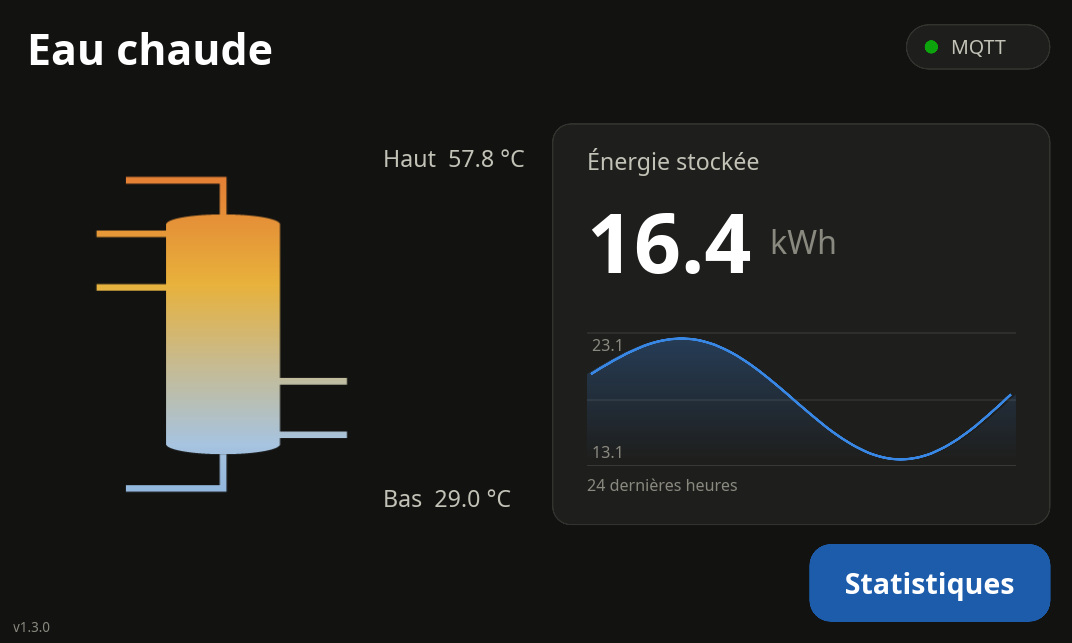
\includegraphics[width=0.48\textwidth]{dashboard.png}\hfill
  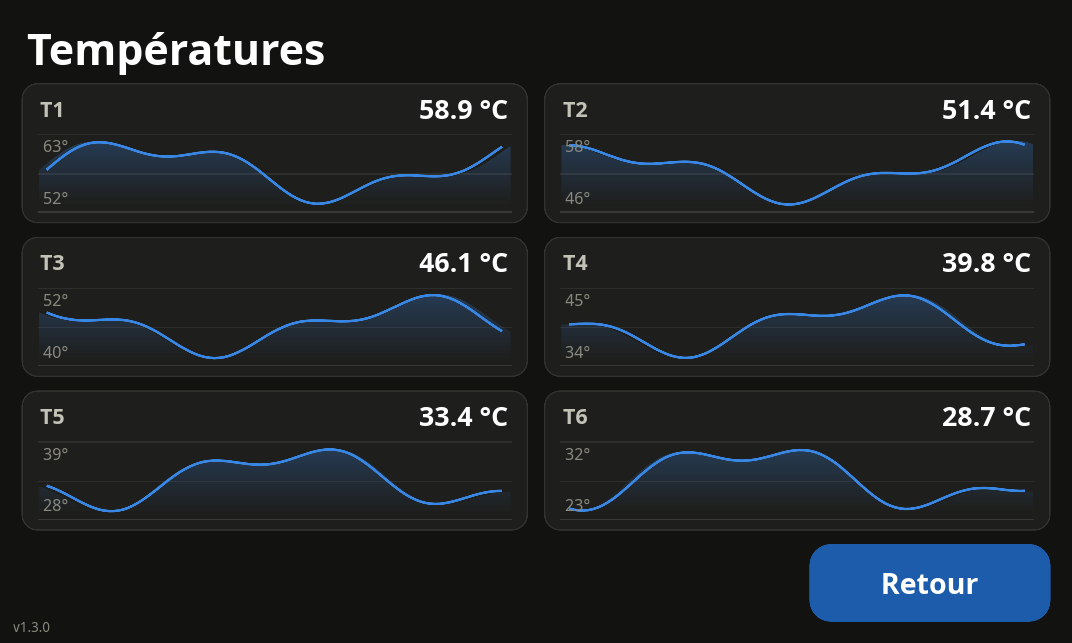
\includegraphics[width=0.48\textwidth]{stats.png}
\end{center}

\textbf{Dashboard} (left): tank drawing colored by the measured
stratification, current top/bottom temperatures, stored energy with its
24-hour history graph. \textbf{Statistics} (right): one card per sensor with
the current value and its auto-scaled 24-hour graph. The buttons at the
bottom right switch between the screens.

\subsection{Status indicators}

\begin{center}
\begin{tabularx}{\textwidth}{@{}lX@{}}
\toprule
\textbf{Indicator} & \textbf{Meaning}\\
\midrule
MQTT chip, green dot & Connected to the broker.\\
MQTT chip, red dot & Broker unreachable; measurements continue, publications resume automatically on reconnection.\\
Amber \enquote{défaut sonde} chip & At least one sensor failed its last reading.\\
Sensor card with red border/value & This sensor is failing; the shown value is the last valid one.\\
Gap in a history graph & Sensor failure or application downtime during that period.\\
\bottomrule
\end{tabularx}
\end{center}

\subsection{History persistence}

The 24-hour histories (one point per 15 minutes, per sensor plus the stored
energy) are saved in \code{history\_file} and restored at startup, shifted by
the downtime. Deleting the file simply restarts the graphs from scratch.
If the \emph{number} of sensors in the configuration changes, the history is
also restarted from scratch --- this is intentional.

% ===========================================================================
\section{Troubleshooting}
% ===========================================================================

\begin{center}
\begin{tabularx}{\textwidth}{@{}lX@{}}
\toprule
\textbf{Symptom} & \textbf{Check}\\
\midrule
No \code{28-*} directory at all &
1-Wire overlay present in \code{config.txt}? Rebooted? Pull-up resistor
fitted? DQ on GPIO4 (pin~7)?\\
\addlinespace
Some sensors missing &
Bus junctions (a single bad crimp drops everything after it); total cable
length; star topology (convert to daisy chain).\\
\addlinespace
Sensor shown in red, \code{crc=... NO} in \code{w1\_slave} &
Electrical noise or loose contact: check the junction of that probe, keep the
bus away from mains cables.\\
\addlinespace
Temperatures look swapped &
Sensor order in \code{config.toml} does not match the physical top-to-bottom
order; redo the mapping of section~\ref{sec:identify}.\\
\addlinespace
MQTT chip stays red &
\code{mqtt.host}/\code{port} correct? Broker reachable
(\code{ping}, \code{mosquitto\_sub})? Firewall?\\
\addlinespace
Energy value seems wrong &
\code{volume\_l} and \code{reference\_temp\_c} correct? All sensors reading
plausibly (Statistics screen)? Thermal contact (a probe reading the room
instead of the wall pulls the value down)?\\
\addlinespace
Window has no titlebar / cannot be closed on a desktop PC &
Intentional (kiosk design). Close with Alt+F4 or \code{kill}.\\
\bottomrule
\end{tabularx}
\end{center}

Useful commands while commissioning:

\begin{lstlisting}[language=bash]
journalctl --user -u boilert -f              # application logs
cat /sys/bus/w1/devices/28-*/w1_slave        # raw sensor readout
mosquitto_sub -h <broker> -t 'boilert/#' -v  # what the broker sees
RUST_LOG=debug ./boilert config.toml         # verbose foreground run
\end{lstlisting}

\subsection{Replacing a sensor}

A new DS18B20 has a new 1-Wire ID:
\begin{enumerate}
  \item Identify the new probe's ID (section~\ref{sec:identify}).
  \item Replace the \code{id} of the corresponding \code{[[sensors]]} entry
        in \code{config.toml} --- keep the same \code{name} and position.
  \item Restart the service: \code{systemctl --user restart boilert}.
\end{enumerate}
Since the sensor \emph{count} is unchanged, the history is preserved; only
the replaced sensor's curve continues with the new probe's data.

\end{document}
